\lchapter{SURF}

\section{Introduction}

SURF (Speeded Up Robust Features) est un descripteur tout comme son prédécesseur SIFT (Scale-Invariant Feature Transform). Son utilité réside dans le fait qu'il est capable de détecter des points d'intérêt sur une image pour ensuite pouvoir effectuer des tâches de reconstruction d'objet en 3D ou de reconnaissance d'objet, le sujet qui nous intéresse.

Son avantage par rapport à SIFT est qu'il est plusieurs fois plus rapides et ses créateurs affirment qu'il est en plus plus robuste aux transformations d'image. Utilisé pour son potentiel de reconnaissance d'objet, SURF nous permet d'extraire des features rapidement et facilement sur une image de caractère afin de pouvoir ensuite les classifier.

Afin de complémenter SURF, nous allons tenter d'utiliser un réseau de neurones pour la classification des caractères. Le choix de SURF s'est principalement basé sur un projet passé ou SURF était utilisé pour sa fonction de reconstruction d'objet 3D. C'était également intéressant pour sortir des sentiers battus.

\section{Environnement}

SURF et le "bag of features" ont été exploités via MATLAB 2014b dans un environnement Windows 8.1 64bits. La gestion des fichiers s'est réalisée via git. Les tests ont été faits sur les caractères 0 à 9 pour les features SURF et sur les caractères 0 à 9 et/ou 0 à z pour "bag of features".

\section{Preprocessing}

Avant de pouvoir aisément travailler avec les images, il a été nécessaire de toutes les convertir en niveaux de gris, afin de ne travailler qu'avec une seule valeur. Un deuxième dataset avec les mêmes images redimensionnées vers le bas a aussi été créé.

\section{Extraction de features SURF}

De mon coté, j'ai suivi deux voies afin d'exploiter les possibilités de SURF. Tout d'abord en utilisant les features que l'on peut extraire via les descripteurs de SURF. En utilisant les méthodes fournies par Matlab (detectSURFFeatures), il est possible d'extraire les points d'intérêt de l'image (example en ure\ref{fig:surffeaturesexample}).

\begin{figure}[h]
\centering
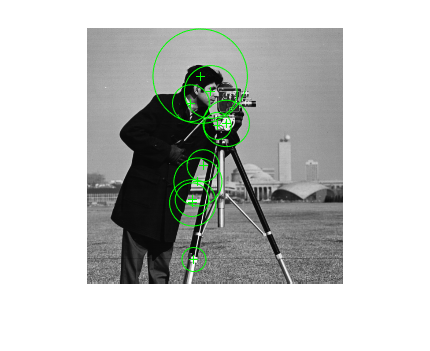
\includegraphics{pictures/DetectSURFFeaturesExample_01.png}
\caption{Points d'intérêt SURF}
\label{fig:surffeaturesexample}
\end{figure}

Après avoir récupéré les points, il est possible d'en extraire les features. Ces features vont dans le cas standard se traduire par un vecteur de taille 64 (un vecteur par point d'intérêt). Ceci est réalisé grâce à la méthode "extractFeatures". Cela va donc créer une matrice qui aura autant de lignes qu'il y a de points et 64 colonnes.

Avant de se lancer dans la classification, il sera néanmoins nécessaire de retravailler un peu ces features, car il n'est pas possible de générer une matrice pour notre réseau de neurones alors que les features sont elle-même déjà des matrices.

Une solution simple est d'aplatir simplement ces matrices de features, ainsi chaque point n'est qu'un morceau du vecteur qui va représenter l'image.

Un autre problème qui se pose est que parfois, certaines images ne possèdent pas assez de points d'intéret par rapport au nombre que l'on spécifie. Une solution a été de simplement ajouter des vecteurs vides afin de palier au manque de lignes de la matrice des features de l'image (qui sera convertie en vecteur je le rappelle).

\section{Classification}

Afin de pouvoir classifier les différents caractères, un réseau de neurones a été choisi. Ce choix vient principalement de la facilité de travailler avec Matlab sur SURF et les réseaux de neurones. Cet environnement m'est également familié.

Chaque image traitée via SURF est devenue une colonne de la matrice et l'ensemble de ces colonnes représentes l'entièreté du dataset (toutes les images). Le système est un système à une couche cachée de type "feed-forward" avec 10 neurones. Certains tests ont été effectués avec différentes valeurs de neurones, sans succès. Le nombre 10 a donc été retenu par défaut.

La toolbox "Neural Net Pattern Recognition" m'a permis d'aller très vite dans le reste du script. En effet, il est possible d'extraire le code très facilement.

\section{Résultats}

Étant donné la nature aléatoire des résultats d'un réseau de neurones (initialisation aléatoire des poids), les résultats ont été considérés en maximum comptabilisé sur 100 runs du script. En effet, lancé le script 2 ou 3 fois peut vous amener à croire que votre réseau est mauvais à 50\%, alors que quelques runs plus tard, il monte à plus de 90\%.

Différents tests ont été effectués avec différents nombres de points d'intérêt : de 5 à 40. Lorsqu'une image n'en avait pas assez, des vecteurs vides ont été rajoutés en guise de feature. 

\begin{figure}[h]
\centering
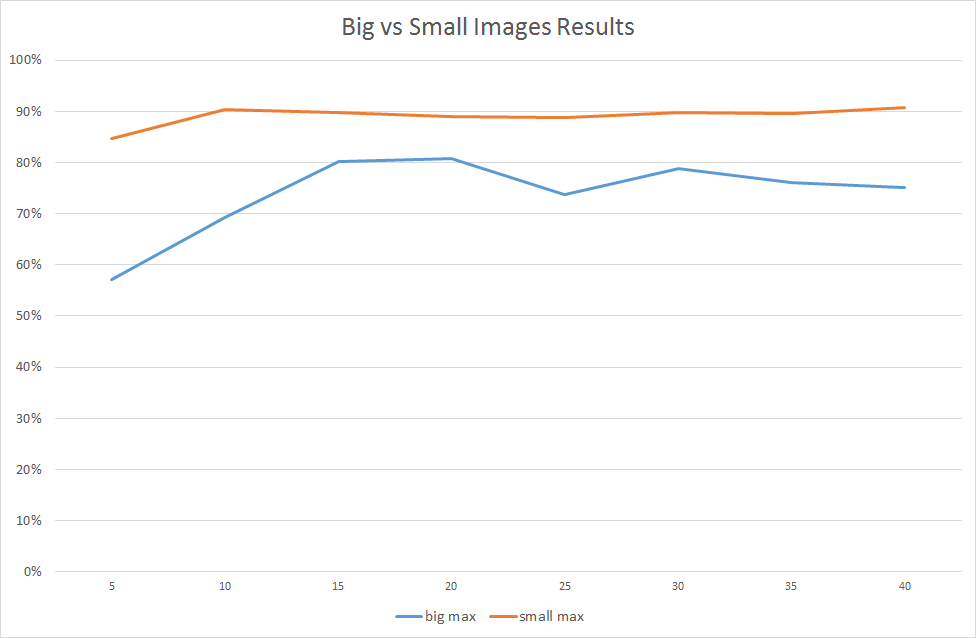
\includegraphics[width=0.8\linewidth]{pictures/bigvssmallresults.png}
\caption{Résultats avec les deux dataset}
\label{fig:resultdataset}
\end{figure}

La \ref{fig:resultdataset} montre les meilleurs résultats obtenus pour chaque nombre de points d'intérêts choisis pour le dataset avec les grandes images ou celles redimensionnées. On peut voir que les résultats avec les petites images sont meilleurs et augmenter le nombre de points au-delà de 10 ne sert é rien. Cela vient certainement du fait que l'on rempli de plus en plus de zéros au fur et à mesure que l'on augmente le nombre de points.

\begin{figure}[h]
\centering
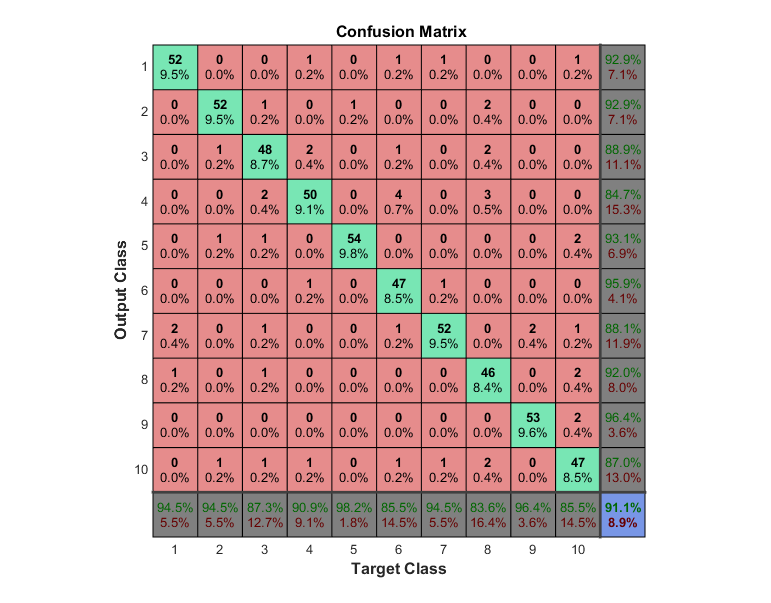
\includegraphics[width=0.8\linewidth]{pictures/small_40_ann_surf.png}
\caption{Matrice de confusion SURF}
\label{fig:confusionmatrice1}
\end{figure}

La \ref{fig:confusionmatrice1} nous montre la matrice de confusion du meilleur résultat avec 40 points d'intérêts sur les petites images. On peut voir certains souci entre le 3, le 5 et le 7 principalement. Le 9 a également du souci avec un peu tout le monde.

\section{Bag of features}

Avant de remplir les points manquants par des vecteurs nuls, le maximum de points que l'on pouvait demander était de 14. En effet, l'une des images n'avait que 14 points d'intérêts. Ceci a posé problème avant la solution des vecteurs nuls et d'autres pistes ont donc été explorées.

Le fait qu'on aplatit la matrice d'une image en 1 seul vecteur est également un traitement pas très propre. Des recherches visant à trouver un moyen de symboliser une image par un seul vecteur de features, la notion de "bag of features" est apparue. Le souci du coté aléatoire des résultats est également résolu.

Le principe du "bag of features" est de créer un vocabulaire avec les features SURF. Toutes ces features vont ensuite être réduites en nombre via une technique de clustering K-means. Finalement, un histogramme de ce vocabulaire pourra servir à représenter l'image et entraîner le classificateur. La classification se déroule au travers d'une SVM linéaire multi classes.

On n'est plus embêté par le nombre de points d'intérêts et les résultats sont plus consistants, ce qui est vraiment pratique.

\section{Résultats}

En parlant de résultats, les résultats atteints avec le "bag of features" sont légèrement meilleures qu'avec les features brutes SURF ( \ref{fig:confusionmatrice2}).

\begin{figure}[h]
\centering
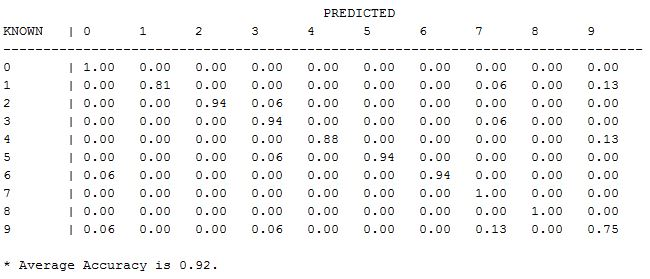
\includegraphics[width=0.8\linewidth]{pictures/bag_confusion_0-9.jpg}
\caption{Matrice de confusion "Bag of features" 0-9}
\label{fig:confusionmatrice2}
\end{figure}

Aux vues des résultats encourageants du "bag of features", j'ai essayé d'ajouter les lettres a à z dans la classification. Cela a fait chuté l'accuracy à 0.87, ce qui est correcte pour 36 classes (\ref{fig:confusionmatrice3}). Le 9 semble à nouveau avoir des problèmes, ici avec le 0 et le 3.

\begin{figure}[h]
\centering
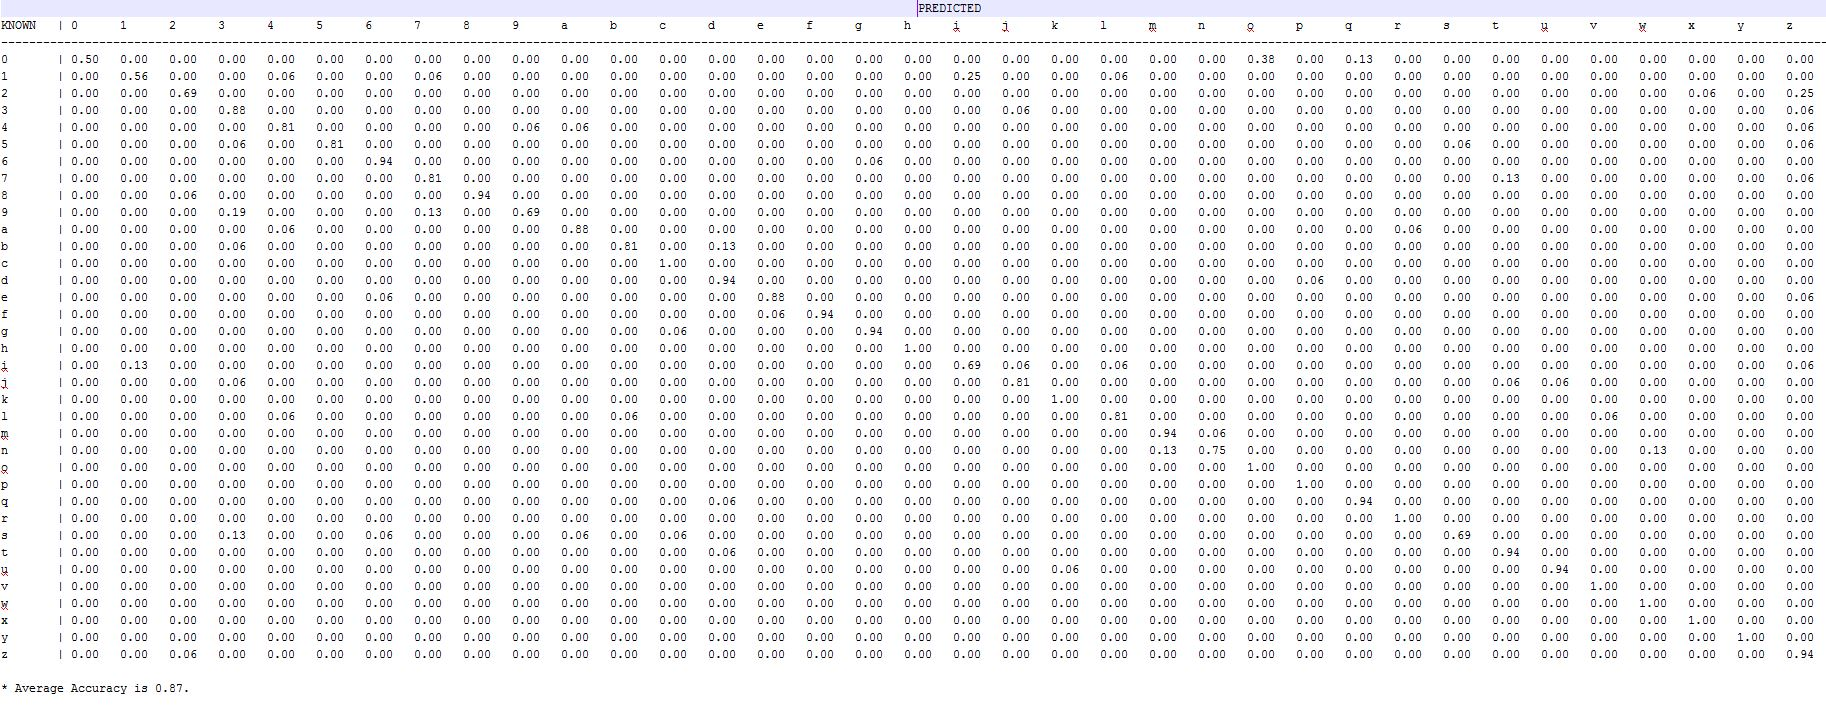
\includegraphics[width=0.8\linewidth]{pictures/bag_confusion_0-z.jpg}
\caption{Matrice de confusion "Bag of features" 0-z}
\label{fig:confusionmatrice3}
\end{figure}

Dans les grandes fautes commises, on peut noter le i et le 1 qui semblent logiques vu leur similarité, mais aussi le s et le 3. Le combo 9/3 est toujours là. Il semble qu'il nécessiterait plus d'attention pour l'optimisation du système.

\section{Problèmes rencontrés}

Les problèmes rencontrés ont tous déjà été cités auparavant :

\begin{itemize}
\item Nombre de points d'intérêts insuffisants avec SURF et donc technique de remplissage avec des vecteurs nuls.
\item Nécessité d'aplatir la matrice des features pour résumer une image à un vecteur. Les vecteurs deviennent vite grands avec une taille de base de 64.
\item Impossibilité d'avoir un score élevé avec tout le dataset (0-9+a-z+A-Z).
\item Problèmes de confusion récurrents, notamment 3/9.
\end{itemize}

\section{Améliorations}

Il y a un point principal à régler afin d'améliorer notre script : le score. Pour cela, la façon la plus simple serait de trouver un moyen de régler les confusions récurrentes (comme 3/9, i/1).

Néanmoins, il y a d'autres routes possibles. On pourrait tenter de se débarrasser de SURF et remplacer cela par autre chose. 

D'autres améliorations possibles serait d'augmenter le nombre de techniques de preprocessing effectué, comme binariser les images en plus de la conversion en niveaux de gris, du thinning, ...